\section{SLURM Architecture}

As a cluster resource manager, SLURM has three key functions.  First,
it allocates exclusive and/or non-exclusive access to resources to users for 
some duration of time so they can perform work.  Second, it provides 
a framework for starting, executing, and monitoring work  
on the set of allocated nodes.  Finally, it arbitrates 
conflicting requests for resources by managing a queue of pending work.
Users and system administrators interact with SLURM using simple commands.

%Users interact with SLURM through four command line utilities: 
%\srun\ for submitting a job for execution and optionally controlling it
%interactively, 
%\scancel\ for early termination of a pending or running job, 
%\squeue\ for monitoring job queues, and 
%\sinfo\ for monitoring partition and overall system state.
%System administrators perform privileged operations through an additional
%command line utility: {\tt scontrol}.
%
%The central controller daemon, {\tt slurmctld}, maintains the global state 
%and directs operations.
%Compute nodes simply run a \slurmd\ daemon (similar to a remote shell 
%daemon) to export control to SLURM.  
%
%SLURM is not a sophisticated batch system.  
%In fact, it was expressly designed to provide high-performance 
%parallel job management while leaving scheduling decisions to an 
%external entity as will be described later. 

\begin{figure}[tb]
\centerline{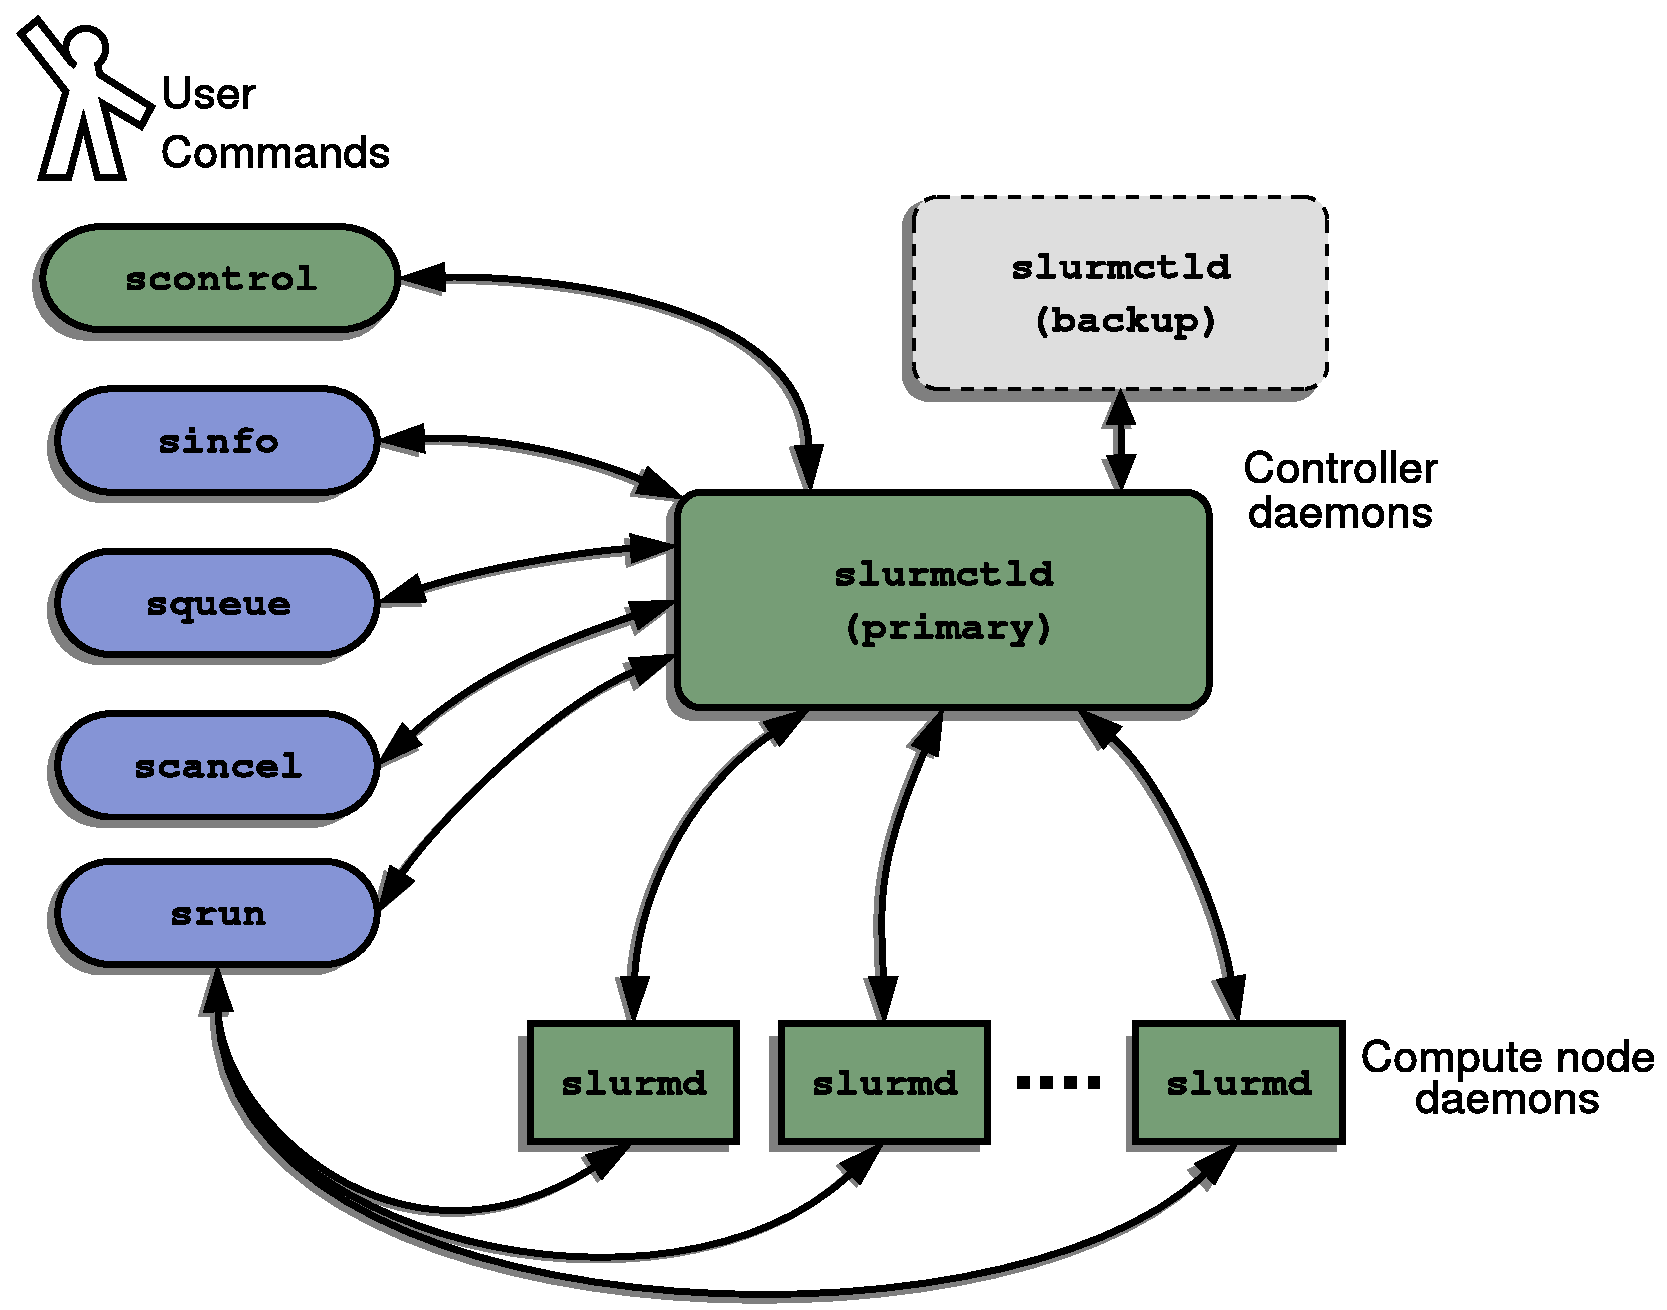
\epsfig{file=../figures/arch.eps,scale=0.40}}
\caption{SLURM Architecture}
\label{arch}
\end{figure}

Figure~\ref{arch} depicts the key components of SLURM. As shown in Figure~\ref{arch},
SLURM consists of a \slurmd\ daemon
running on each compute node, a central \slurmctld\ daemon running on
a management node (with optional fail-over twin), and five command line
utilities,
% {\tt srun}, {\tt scancel}, {\tt sinfo}, {\tt squeue}, and {\tt scontrol}, 
which can run anywhere in the cluster.  

The entities managed by these SLURM daemons include nodes, the
compute resource in SLURM, partitions, which group nodes into
logical disjoint sets, jobs, or allocations of resources assigned
to a user for a specified amount of time, and job steps, which are
sets of tasks within a job.  
Each job is allocated nodes within a single partition. 
Once a job is assigned a set of nodes, the user is able to initiate
parallel work in the form of job steps in any configuration within the
allocation. For instance a single job step may be started which utilizes
all nodes allocated to the job, or several job steps may independently 
use a portion of the allocation.

%\begin{figure}[tcb]
%\centerline{\epsfig{file=../figures/entities.eps,scale=0.7}}
%\caption{SLURM Entities}
%\label{entities}
%\end{figure}
%
%Figure~\ref{entities} further illustrates the interrelation of these
%entities as they are managed by SLURM. The diagram shows a group of
%compute nodes split into two partitions. Partition 1 is running one
%job, with one job step utilizing the full allocation of that job.
%The job in Partition 2 has only one job step using half of the original
%job allocation.
%That job might initiate additional job step(s) to utilize 
%the remaining nodes of its allocation.

\begin{figure}[tb]
\centerline{\epsfig{file=../figures/slurm-arch.eps,scale=0.5}}
\caption{SLURM Architecture - Subsystems}
\label{archdetail}
\end{figure}

Figure~\ref{archdetail} exposes the subsystems that are implemented
within the \slurmd\ and \slurmctld\ daemons.  These subsystems
are explained in more detail below.

\subsection{SLURM Local Daemon (Slurmd)}

The \slurmd\ is a multi-threaded daemon running on each compute node.
It reads the common SLURM configuration file and recovers any 
previously saved state information, 
notifies the controller that it is active, waits for work, 
executes the work, returns status, and waits for more work.  
Since it initiates jobs for other users, it must run with root privilege.
%It also asynchronously exchanges node and job status information with {\tt slurmctld}.  
The only job information it has at any given time pertains to its 
currently executing jobs.
The \slurmd\ performs five major tasks.

\begin{itemize}
\item {\em Machine and Job Status Services}:  Respond to controller 
requests for machine and job state information, and send asynchronous 
reports of some state changes (e.g. \slurmd\ startup) to the controller.

\item {\em Remote Execution}: Start, monitor, and clean up after a set
of processes (typically belonging to a parallel job) as dictated by the
\slurmctld\ daemon or an \srun\ or \scancel\ command. Starting a process may
include executing a prolog program, setting process limits, setting real
and effective user id, establishing environment variables, setting working
directory, allocating interconnect resources, setting core file paths,
initializing the Stream Copy Service, and managing
process groups. Terminating a process may include terminating all members
of a process group and executing an epilog program.

\item {\em Stream Copy Service}: Allow handling of stderr, stdout, and
stdin of remote tasks. Job input may be redirected from a file or files, a
\srun\ process, or /dev/null.  Job output may be saved into local files or
sent back to the \srun\ command. Regardless of the location of stdout or stderr,
all job output is locally buffered to avoid blocking local tasks.

\item {\em Job Control}: Allow asynchronous interaction with the
Remote Execution environment by propagating signals or explicit job
termination requests to any set of locally managed processes.

\end{itemize}

\subsection{SLURM Central Daemon (Slurmctld)}

Most SLURM state information is maintained by the controller, {\tt slurmctld}.
The \slurmctld\ is multi-threaded with independent read and write locks 
for the various data structures to enhance scalability. 
When \slurmctld\ starts, it reads the SLURM configuration file.  
It can also read additional state information
from a checkpoint file generated by a previous execution of {\tt slurmctld}.
Full controller state information is written to 
disk periodically with incremental changes written to disk immediately
for fault-tolerance.  
The \slurmctld\ runs in either master or standby mode, depending on the
state of its fail-over twin, if any.
The \slurmctld\ need not execute with root privilege.
%In fact, it is recommended that a unique user entry be created for 
%executing \slurmctld\ and that user must be identified in the SLURM 
%configuration file as {\tt SlurmUser}.
The \slurmctld\ consists of three major components:

\begin{itemize}
\item {\em Node Manager}: Monitors the state of each node in
the cluster.  It polls {\tt slurmd}'s for status periodically and
receives state change notifications from \slurmd\ daemons asynchronously.
It ensures that nodes have the prescribed configuration before being 
considered available for use.

\item {\em Partition Manager}: Groups nodes into non-overlapping sets called
{\em partitions}. Each partition can have associated with it various job
limits and access controls.  The partition manager also allocates nodes
to jobs based upon node and partition states and configurations. Requests
to initiate jobs come from the Job Manager.  The \scontrol\ may be used
to administratively alter node and partition configurations.

\item {\em Job Manager}: Accepts user job requests and places pending 
jobs in a priority ordered queue. 
The Job Manager is awakened on a periodic basis and whenever there
is a change in state that might permit a job to begin running, such
as job completion, job submission, partition-up transition,
node-up transition, etc.  The Job Manager then makes a pass
through the priority-ordered job queue. The highest priority jobs 
for each partition are allocated resources as possible. As soon as an 
allocation failure occurs for any partition, no lower-priority jobs for 
that partition are considered for initiation. 
After completing the scheduling cycle, the Job Manager's scheduling
thread sleeps.  Once a job has been allocated resources, the Job Manager
transfers necessary state information to those nodes, permitting it 
to commence execution.  When the Job Manager detects that
all nodes associated with a job have completed their work, it initiates
clean-up and performs another scheduling cycle as described above.

\end{itemize}
